\documentclass[11pt,aspectratio=169]{beamer}

\usetheme{Boadilla}
\usecolortheme{default}
\setbeamertemplate{navigation symbols}{}
\setbeamertemplate{itemize item}{\small$\blacktriangleright$}
%\setbeameroption{show notes on second screen=right}
\setbeameroption{hide notes}

\usepackage{amsmath,amssymb,amsfonts,mathtools}
\usepackage{bm}
\usepackage{booktabs}
\usepackage{graphicx}
\usepackage{tikz}
\usetikzlibrary{shapes.geometric}
\usepackage{enumerate}

\definecolor{BerkeleyBlue}{RGB}{0,50,98}
\definecolor{BerkeleyGold}{RGB}{253,181,21}
\setbeamercolor{title}{fg=BerkeleyBlue}
\setbeamercolor{frametitle}{fg=BerkeleyBlue}
\setbeamercolor{structure}{fg=BerkeleyBlue}
\setbeamercolor{alerted text}{fg=BerkeleyBlue}

\newcommand{\Pbb}{\mathbb{P}}
\newcommand{\Ebb}{\mathbb{E}}
\newcommand{\Nbb}{\mathbb{N}}
\newcommand{\gij}[3]{g_{#1,#2}(#3)}

\title[Bipartition Cover Bounds under MSC]{Bipartition Covers in the Multispecies Coalescent Model}
\author{Zachary McNulty}
\institute{UC Berkeley}
\date{UC Berkeley Probability Seminar \\ March 4, 2026}

\begin{document}

\begin{frame}
  \titlepage
\note{
  Hello everyone, my name is Zachary McNulty and today I will be talking about this neat little project I worked on last semester.
  The focus will be on these things called bipartition covers, which appear naturally in the context of phylogenetic inference under the multispecies coalescent model.
  Thanks to Steve for all his help and guidance, and without further ado, let's get rolling. 

}
\end{frame}

\begin{frame}{Talk Outline}

\begin{itemize}
  \item Background: phylogenetic inference and MSC model
  \item Motivation: superexponential tree search and bipartition covers
  \item Identify worst-case topologies and a balancing lemma.
   \item Empirical results
  \item Asymptotic analysis

\end{itemize}
\note{
  Here's a brief roadmap of what I plan on talking about today. We will start with some background on some of the goals and challenges of phylogenetic inference, 
  and then introduce the core mathematical model underlying this talk: the multispecies coalescent model. \\
  
  \vspace{0.5em}
  Then we will talk about the motivation for this project, 
  which is to try to get around this superexponentail tree search space  that appears in these inference procedures, and the main tool
  --bipartition covers--that we will try to use to do so. \\

  \vspace{0.5em}
  At the end of the day, we will try to develop bound on how much data you need for this bipartition cover approach to work, and we will try to identify 
  some of the "worst-cases" which make phylogenetic inference difficult.\\
  
  \vspace{0.5em}
  Later on, we will discuss some asymptotics of how these 
  bounds perform in some natural parameter regimes, and lastly provide some empirical results showing how they behave in practice at finite-samples.
}
\end{frame}

\section{Setup}


%%%%%%%%%%%%%%%%%%%%%%%%%%%%%%%%%%%%%%%%
% Background %
%%%%%%%%v%%%%%%%%%%%%%%%%%%%%%%%%%%%%%%%%

\begin{frame}{Background: Phylogenetic Inference}

\textbf{Goal:} Given a collection of $k$ species, estimate their evolutionary history (\textit{species tree})

\begin{center}
  \begin{minipage}{0.31\linewidth}
    \centering
    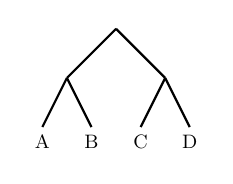
\begin{tikzpicture}[scale=0.78, transform shape, thick, every node/.style={font=\small}]
      \coordinate (r) at (0,1.4);
      \coordinate (u) at (-0.8,0.6);
      \coordinate (d) at (0.8,0.6);
      \coordinate (a) at (-1.2,-0.2);
      \coordinate (b) at (-0.4,-0.2);
      \coordinate (c) at (0.4,-0.2);
      \coordinate (e) at (1.2,-0.2);

      \draw (r) -- (u);
      \draw (r) -- (d);
      \draw (u) -- (a);
      \draw (u) -- (b);
      \draw (d) -- (c);
      \draw (d) -- (e);

      \node[below] at (a) {A};
      \node[below] at (b) {B};
      \node[below] at (c) {C};
      \node[below] at (e) {D};
    \end{tikzpicture}
  \end{minipage}
  \hfill
  \begin{minipage}{0.31\linewidth}
    \centering
    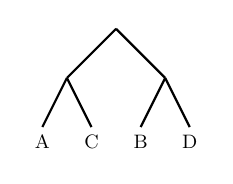
\begin{tikzpicture}[scale=0.78, transform shape, thick, every node/.style={font=\small}]
      \coordinate (r) at (0,1.4);
      \coordinate (u) at (-0.8,0.6);
      \coordinate (d) at (0.8,0.6);
      \coordinate (a) at (-1.2,-0.2);
      \coordinate (b) at (-0.4,-0.2);
      \coordinate (c) at (0.4,-0.2);
      \coordinate (e) at (1.2,-0.2);

      \draw (r) -- (u);
      \draw (r) -- (d);
      \draw (u) -- (a);
      \draw (u) -- (b);
      \draw (d) -- (c);
      \draw (d) -- (e);

      \node[below] at (a) {A};
      \node[below] at (b) {C};
      \node[below] at (c) {B};
      \node[below] at (e) {D};
    \end{tikzpicture}
  \end{minipage}
  \hfill
  \begin{minipage}{0.31\linewidth}
      \centering
      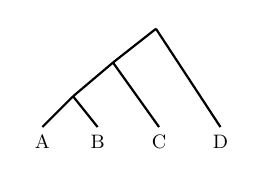
\begin{tikzpicture}[scale=0.78, transform shape, thick, every node/.style={font=\small}]
      % Caterpillar in the same style as the Extremal Topologies slide
      \coordinate (r) at (0,1.4);
      \coordinate (n1) at (-0.7,0.85);
      \coordinate (n2) at (-1.35,0.30);
      \coordinate (a) at (-1.85,-0.2);
      \coordinate (b) at (-0.95,-0.2);
      \coordinate (c) at (0.05,-0.2);
      \coordinate (d) at (1.05,-0.2);

      \draw (r) -- (n1);
      \draw (r) -- (d);
      \draw (n1) -- (n2);
      \draw (n1) -- (c);
      \draw (n2) -- (a);
      \draw (n2) -- (b);

      \node[below] at (a) {A};
      \node[below] at (b) {B};
      \node[below] at (c) {C};
      \node[below] at (d) {D};
    \end{tikzpicture}
  \end{minipage}
\end{center}

\vspace{1em}
\noindent \textbf{Challenge:} We only have modern day DNA sequences, not the actual evolutionary history.



\note{
  Let's start by introducing what phylogenetic inference is. The goal is to estimate the evolutionary history 
  of a collection of species, which we can represent as a tree. Here I have four species, which I label $A,B,C,D$, 
  and I have three different trees which represent three different possible evolutionary histories for these species.
  Our goal is to somehow determine which history is most likely given whatever data we have available.\\

  \vspace{0.5em}

  \noindent The challenge of course is we have no access to the actual evolutionary history, 
  and instead have to infer it from what data is available about species in the modern day. DNA of course
  is of course one of the most abundant and informative sources of such data.
}
\end{frame}

% Background: phylogenetic inference 2
\begin{frame}{Background: Phylogenetic Inference}

\noindent In \textit{consensus methods}, this occurs in two stages: 
\begin{itemize}
  \item For each gene, generate an estimate of its evolutionary history (\textit{gene tree}).
  \item Aggregate these into a single estimate of the species tree.
\end{itemize}

\begin{center}
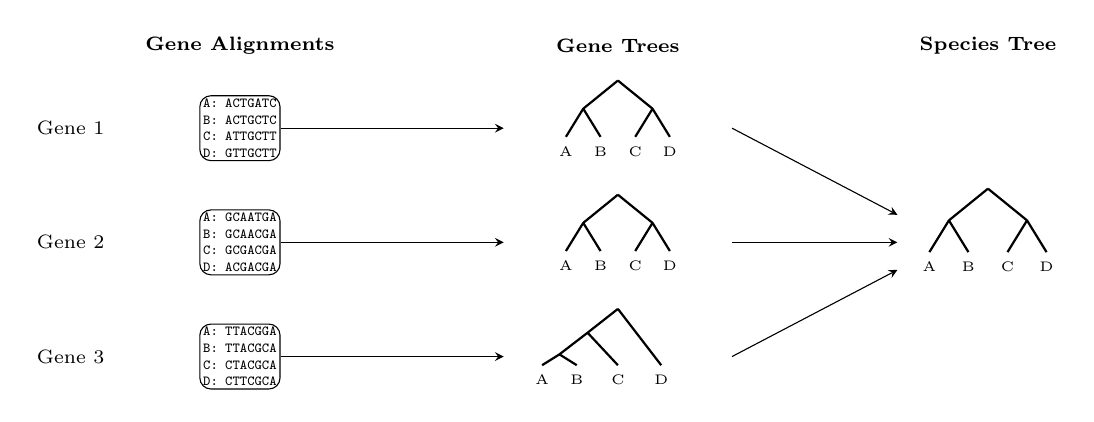
\begin{tikzpicture}[x=1cm,y=1cm,>=stealth]
  % Column headers
  \node[font=\scriptsize\bfseries] at (-4.8,2.5) {Gene Alignments};
  \node[font=\scriptsize\bfseries] at (0,2.5) {Gene Trees};
  \node[font=\scriptsize\bfseries] at (4.7,2.5) {Species Tree};

  % Row labels
  \node[font=\scriptsize] at (-6.95,1.45) {Gene 1};
  \node[font=\scriptsize] at (-6.95,0.00) {Gene 2};
  \node[font=\scriptsize] at (-6.95,-1.45) {Gene 3};

  % Left column: mock DNA alignments
  \node[draw, rounded corners, align=left, font=\ttfamily\tiny, inner sep=1.2pt] (seq1) at (-4.8,1.45)
    {A: ACTGATC\\B: ACTGCTC\\C: ATTGCTT\\D: GTTGCTT};
  \node[draw, rounded corners, align=left, font=\ttfamily\tiny, inner sep=1.2pt] (seq2) at (-4.8,0.00)
    {A: GCAATGA\\B: GCAACGA\\C: GCGACGA\\D: ACGACGA};
  \node[draw, rounded corners, align=left, font=\ttfamily\tiny, inner sep=1.2pt] (seq3) at (-4.8,-1.45)
    {A: TTACGGA\\B: TTACGCA\\C: CTACGCA\\D: CTTCGCA};

  % Middle column: three gene-tree topologies
  \begin{scope}[shift={(0,1.45)},scale=0.55,thick]
    \coordinate (r) at (0,1.1);
    \coordinate (u) at (-0.8,0.45);
    \coordinate (d) at (0.8,0.45);
    \coordinate (a) at (-1.2,-0.2);
    \coordinate (b) at (-0.4,-0.2);
    \coordinate (c) at (0.4,-0.2);
    \coordinate (e) at (1.2,-0.2);
    \draw (r)--(u) (r)--(d) (u)--(a) (u)--(b) (d)--(c) (d)--(e);
    \node[below, font=\tiny] at (a) {A};
    \node[below, font=\tiny] at (b) {B};
    \node[below, font=\tiny] at (c) {C};
    \node[below, font=\tiny] at (e) {D};
  \end{scope}

  \begin{scope}[shift={(0,0)},scale=0.55,thick]
    \coordinate (r) at (0,1.1);
    \coordinate (u) at (-0.8,0.45);
    \coordinate (d) at (0.8,0.45);
    \coordinate (a) at (-1.2,-0.2);
    \coordinate (b) at (-0.4,-0.2);
    \coordinate (c) at (0.4,-0.2);
    \coordinate (e) at (1.2,-0.2);
    \draw (r)--(u) (r)--(d) (u)--(a) (u)--(b) (d)--(c) (d)--(e);
    \node[below, font=\tiny] at (a) {A};
    \node[below, font=\tiny] at (b) {B};
    \node[below, font=\tiny] at (c) {C};
    \node[below, font=\tiny] at (e) {D};
  \end{scope}

  \begin{scope}[shift={(0,-1.45)},scale=0.55,thick]
    \coordinate (r) at (0,1.1);
    \coordinate (n1) at (-0.7,0.55);
    \coordinate (n2) at (-1.35,0.05);
    \coordinate (a) at (-1.75,-0.2);
    \coordinate (b) at (-0.95,-0.2);
    \coordinate (c) at (0.00,-0.2);
    \coordinate (d) at (1.00,-0.2);
    \draw (r)--(n1) (r)--(d) (n1)--(n2) (n1)--(c) (n2)--(a) (n2)--(b);
    \node[below, font=\tiny] at (a) {A};
    \node[below, font=\tiny] at (b) {B};
    \node[below, font=\tiny] at (c) {C};
    \node[below, font=\tiny] at (d) {D};
  \end{scope}

  % Right column: single species tree in center row only
  \begin{scope}[shift={(4.7,0)},scale=0.62,thick]
    \coordinate (r) at (0,1.1);
    \coordinate (u) at (-0.8,0.45);
    \coordinate (d) at (0.8,0.45);
    \coordinate (a) at (-1.2,-0.2);
    \coordinate (b) at (-0.4,-0.2);
    \coordinate (c) at (0.4,-0.2);
    \coordinate (e) at (1.2,-0.2);
    \draw (r)--(u) (r)--(d) (u)--(a) (u)--(b) (d)--(c) (d)--(e);
    \node[below, font=\tiny] at (a) {A};
    \node[below, font=\tiny] at (b) {B};
    \node[below, font=\tiny] at (c) {C};
    \node[below, font=\tiny] at (e) {D};
  \end{scope}

  % Flow arrows
  \draw[->] (seq1.east) -- (-1.45,1.45);
  \draw[->] (seq2.east) -- (-1.45,0.00);
  \draw[->] (seq3.east) -- (-1.45,-1.45);
  \draw[->] (1.45,1.45) -- (3.55,0.35);
  \draw[->] (1.45,0.00) -- (3.55,0.00);
  \draw[->] (1.45,-1.45) -- (3.55,-0.35);
\end{tikzpicture}
\end{center}
  

\note{
  One method for doing this is known as \textit{consensus methods}. Here we collect the DNA sequences from a bunch of different genes that all the species
  share. We then use the following two step procedure: first, for each gene, we generate an estimate of its evolutionary history, which we call a \textit{gene tree}, using some
  model of how DNA evolves over time. Each gene tells a possibly different evolutionary story, and these are the things we can actually estimate. 
  Next, since we believe these individual gene histories are in some way influenced by the evolutionary tree of the species, we hope we can aggregate these gene trees into a 
  single estimate of the species tree.\\

  \vspace{0.5em}

  I have a diagram illustrating this procedure here. We start with a collection of DNA sequences for each gene, which we use to estimate a gene tree for each gene. Here the first two genes agree on the evolutionary history, while the latter does not. 
  We then hope to somehow reconcile these gene trees into a single species tree. For example, here we might just take the modal tree as our estimate (in practice this is not generally a good idea, but for illustrative purposes its nice).

  \vspace{0.5em}
  In our talk, we are exclusively interested in the second step of this procedure, which is the aggregation step. 
  As we make precise below, we will sort of assume that we have perfect estimates of the gene trees, ignoring this first estimation step, and we will try to understand how to best use these gene trees to estimate the species tree
  in this aggregation step.
}


\end{frame}


% Background: Kingmans coalescent
\begin{frame}{Background: Kingman's Coalescent}

\begin{figure}[scale=0.7]
  \centering
    \includegraphics[width=0.6\linewidth,height=0.52\textheight]{figures/Kingman_coalescent.png}
  \caption{Kingman's coalescent process: Adwiladan, CC BY-SA 4.0, via Wikimedia Commons.}
\end{figure}

Start with $n$ lineages. Each pair of lineages coalesces at rate one. 

\note{

  \noindent Okay we want to make precise the model we are working with, and what sort of information these gene trees 
  contain about the species tree.\\

  \vspace{0.5em}
  
  To start, we introduce Kingman's coalescent, which is sort of the simplest model for a coalescing process and genealogy you can have. 
  Its described as follows: if there are $n$ lineages currently present, then each of the ${n \choose 2}$ pairs coalesce at rate one. 
  This gives a total coalescence rate of ${n \choose 2}$ when we have $n$ lineages, giving it strong coalescent properties when $n$ is large. \\

  \vspace{0.5em}
  While this model seems simple at first, it actually quite robust and reasonable. It has strong universality properties, in the sense
  that there are many biologically reasonable forward-time population models whose genealogies converge to Kingman's coalescent in the large population limit.
  
  \vspace{0.5em}
  
  Moreover, it has a slew of convenient mathematical properties that make it quite tractable. For one, its Markovian, so it has a strong
  memoryless property. It also has the interesting property that it comes down from infinity, meaning that if we start with infinitely many lineages, 
  we will have only finitely many lineages after any positive amount of time. So its coalescencing properties are very strong. 

}

\end{frame}

\begin{frame}{Background: Multispecies Coalescent Model}

\begin{center}
  \includegraphics[width=0.6\linewidth]{figures/msc_model.PNG}
\end{center}

\smallskip
\noindent The \textit{multispecies coalescent model (MSC)} models gene trees directly.
\begin{itemize}
  \item Along each branch, each pair of lineages coalesce at rate one (Kingman's coalescent)
  \item Gene tree topologies can differ from species tree.
\end{itemize}

\note{
  Now we introduce the multispecies coalescent model, which makes precise what we mean by the gene trees being influenced by the species tree.
  Again, this allows us to sort of directly model the gene trees, skipping this first estimation step and cutting out the modeling of DNA evolution entirely. 
  In this way, we sort of treat the estimation problem of gene trees as solved, and assume we just have
  these correct gene trees as our inputs.\\

  \vspace{0.5em}
  
  The MSC assumes that gene lineages coalesce according to Kingman's coalescent, but are in a sense constrained by the species tree.
  Namely, lineages can only coalesce when they are in the same branch of the species tree, and they must exit a branch before they can coalesce with lineages from other branches. 
  (do an example pointing at the diagram)\\

  \vspace{0.5em}

  The key observation is that gene tree topologies can differ from the species tree, and that the MSC provides a nice model for how they differ while still being informative about the species tree.
}
\end{frame}

\begin{frame}{Motivation: Search-Space Bottleneck}
Many consensus methods are framed as optimization problems over the space of trees:
%
\[\hat{\mathcal{T}} = \arg\max_{\mathcal{T}} \mathrm{support}(\mathcal{T}, \mathcal{G}) \] 
%
\noindent \textbf{Issue:} There are $(2k-3)!!$ possible rooted binary phylogenetic trees.

\begin{itemize}
  \item At $k=20$ this is $\approx 8.2 \times 10^{21}$.
  \item We must find some way to restrict search space.
\end{itemize}

\note{
  Now we are ready to introduce the problem we actually solve. Given a set $\mathcal{G}$ of gene trees, many
  consensus methods are framed as optimization problems over the search space of trees. Here $\mathrm{support}$ is some measure of how "aligned" 
  a given species tree is with the given collection $\mathcal{G}$ of gene trees.\\

  \vspace{0.5em}
  The main obstacle is that this search space is huge. There are $(2k-3)!!$ possible rooted binary phylogenetic trees on $k$ leaves, which grows superexponentially in $k$.
  For example, at $k=20$ this is approximately $8.2 \times 10^{21}$ trees. To make this problem tractable for more than a handful of species, we must 
  find some way of restricting the search space.\\

  \vspace{0.5em}

  Of course, the key insight is thatalmost all of these phylogenetic trees are completely at odds with our gene trees. So we want to
  try to use our gene trees to inform where in this search space the species tree likely lies.
}
\end{frame}

\begin{frame}{Motivation: Bipartition Covers}


  Every edge $e$ in a tree $\mathcal{T}$ generates a \textit{bipartition} $A \mid B$ of its leaves.

\begin{center}
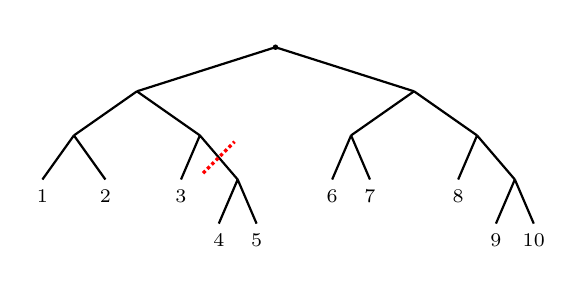
\begin{tikzpicture}[x=0.8cm,y=0.8cm,thick,every node/.style={font=\scriptsize}]
  % Internal nodes
  \coordinate (r) at (0,2.0);
  \coordinate (L) at (-2.2,1.3);
  \coordinate (R) at (2.2,1.3);
  \coordinate (L1) at (-3.2,0.6);
  \coordinate (L2) at (-1.2,0.6);
  \coordinate (L3) at (-0.6,-0.1);
  \coordinate (R1) at (1.2,0.6);
  \coordinate (R2) at (3.2,0.6);
  \coordinate (R3) at (3.8,-0.1);

  % Leaves (10 taxa)
  \coordinate (x1) at (-3.7,-0.1);
  \coordinate (x2) at (-2.7,-0.1);
  \coordinate (x3) at (-1.5,-0.1);
  \coordinate (x4) at (-0.9,-0.8);
  \coordinate (x5) at (-0.3,-0.8);
  \coordinate (x6) at (0.9,-0.1);
  \coordinate (x7) at (1.5,-0.1);
  \coordinate (x8) at (2.9,-0.1);
  \coordinate (x9) at (3.5,-0.8);
  \coordinate (x10) at (4.1,-0.8);

  % Tree edges
  \draw (r)--(L) (r)--(R);
  \draw (L)--(L1) (L)--(L2);
  \draw (L1)--(x1) (L1)--(x2);
  \draw (L2)--(x3) (L2)--(L3);
  \draw (L3)--(x4) (L3)--(x5);
  \draw (R)--(R1) (R)--(R2);
  \draw (R1)--(x6) (R1)--(x7);
  \draw (R2)--(x8) (R2)--(R3);
  \draw (R3)--(x9) (R3)--(x10);

  % Root and labels
  \fill (r) circle (1pt);
  \node[above] at (r) {};
  \node[below] at (x1) {$1$};
  \node[below] at (x2) {$2$};
  \node[below] at (x3) {$3$};
  \node[below] at (x4) {$4$};
  \node[below] at (x5) {$5$};
  \node[below] at (x6) {$6$};
  \node[below] at (x7) {$7$};
  \node[below] at (x8) {$8$};
  \node[below] at (x9) {$9$};
  \node[below] at (x10) {$10$};

  % A cut crossing one branch
  \draw[red,densely dotted,very thick] (-1.15,0.00) -- (-0.65,0.50);
\end{tikzpicture}
\end{center}

\begin{center}
  \footnotesize The bipartition associated to the highlighted edge is $\{4,5\} \cup \{1,2,3,6,7,8,9,10\}$.
\end{center}


Denote $\Sigma(\mathcal{T})$ the set of bipartitions. We say a set $\mathcal{G}$ of trees forms a \textit{bipartition cover} if:

\[\Sigma(\mathcal{T}) \subseteq \bigcup_{g \in \mathcal{G}} \Sigma(g)\]

\note{
  Let's introduce one way in which this restriction can be done, which motivated this current project.
  Given a phylogenetic tree $\mathcal{T}$, every edge $e$ in $\mathcal{T}$ induces a bipartition of the leaves of $\mathcal{T}$. 
  In a rooted tree, this is the set of leaves below $e$ and the set of leaves not below $e$. Here we have a picture illustrating one such bipartition.\\

  \vspace{0.5em}
  \noindent Denote $\Sigma(\mathcal{T})$ the set of bipartitions of $\mathcal{T}$. It is not hard to see that $\Sigma(\mathcal{T})$ characterizes $\mathcal{T}$, 
  in the sense that if you know the set of bipartitions of a tree, you can reconstruct the tree itself. This is a result known as Buneman's splits-equivalence theorem.
  Hence these objects are quite natural.\\

  \vspace{0.5em}
  We say a set $\mathcal{G}$ of trees forms a \textit{bipartition cover} if every bipartition of $\mathcal{T}$ is present in at least one of the trees in $\mathcal{G}$. Namely if
  the union of the sets of bipartitions of the trees in $\mathcal{G}$ contains the set of bipartitions of $\mathcal{T}$.
}
\end{frame}

\begin{frame}{Problem Setting}

  \noindent \textbf{Idea:} consider only species trees whose bipartitions are present in the gene trees.

  \vspace{0.25in}
  Namely, we restrict our search space to:
  %
  \[\mathcal{A} := \bigg\{\mathcal{T} \; : \; \Sigma(\mathcal{T}) \subseteq \bigcup_{g \in \mathcal{G}} \Sigma(g)\bigg\}\]
  %
  \noindent \textbf{Our Question:} How many genes are required to ensure $\mathcal{T}^* \in \mathcal{A}$ with high probability?

\note{
  This characterization of trees by their bipartitions suggests a natural way to restrict the search space: we can consider only species trees whose bipartitions are present in the gene trees.\\

  \vspace{0.5em}

  With this in mind, it is natural to ask: how much data do we need so that the species tree is in this restricted search space with
  high probability? This question was the main focus of this project.
}
\end{frame}

\begin{frame}{Project goals}

  In this project, we aim to develop:
  \begin{itemize}
    \item Topology-free bounds on coverage probability $\mathbb{P}(\mathcal{T}\in \mathcal{A})$.
    \item Deeper understanding of ``worst-case'' topologies under MSC.
    \item Asympototic analysis of absorption times in Kingman's coalescent.
  \end{itemize}
\note{
  Let's go over some goals of this project. \\

  \vspace{0.5em}

  First, we of course want to develop bounds on the coverage probability we just introduced. 
  Since species tree is unknown at inference time, we would like to utilize as little information about 
  the species tree as possible. In particular, we won't assume anything about its topology. As we will discuss below,
  the only assumptions we will make will be about the minimal branch length of the species tree. Its easy to see without this,
  no such bounds are possible: in the limit as $T_{min} \to 0$, the gene trees are completely uninformative about the species tree, and so no bounds are possible.\\

  \vspace{0.5em}

  In order to develop these bounds, we will need to understand what topologies make inference the "most difficult" under the MSC, and why these
  produce bottlenecks. This will be the main focus of the first half of the talk.\\

  \vspace{0.5em}

  Lastly, since our bounds are semi-complicated functions of the given parameters, we will want to understand how they behave in some natural asymptotic regimes. 
  This will be the main focus of the second half of the talk.\\
}
\end{frame}

\begin{frame}{Key Coalescent Probability}
For $1 \leq j \leq i$, define:
%
\begin{align*}
\gij{i}{j}{t}& =\Pbb(\text{$i$ lineages coalesce into $j$ after time $t$ under Kingman's coalescent})\\
             & = \sum_{k=j}^i \frac{e^{-{k \choose 2}t} (2k-1)(-1)^{k-j}j_{(k-1)} i_{[k]}}{j!(k-j)!i_{(k)}}
\end{align*}

In particular, $\gij{\ell}{1}{t}$ is the probability for full coalescence of $\ell$ lineages by time $t$.

\vspace{0.6em}
\textbf{Properties $\gij{\ell}{1}{t}$:}
\begin{itemize}
  \item Increasing, log-concave in $t$. Decreasing, convex in $\ell$.  
  \item Can view as the CDF of $\sum_{i=2}^{\ell} \mathrm{Exp}\left({i \choose 2}\right)$.
  \item Bound away from zero: $s(t) := \lim_{\ell \to \infty}  \gij{\ell}{1}{t} > 0$. 
\end{itemize}
\note{
  We start by defining these coalescent probabilities under Kingman's coalescent.


  \vspace{0.5em}
  Since the MSC is just a structured version of Kingman's coalescent, its maybe unsurprising
  that all our bounds will be framed in terms of these coalescent probabilities. 
  In particular, the key probability we will be interested in is the absorption probability $\gij{\ell}{1}{t}$, 
  which is the probability that $\ell$ lineages coalesce into one by time $t$. \\

  \vspace{0.5em}
  These absorption probabilities have some convenient properties. They have nice monotonicity and
  concavity properties in both $t$ and $\ell$. Moreover, since there's an exponential waiting time between
  each coalescent event, this is literally just the CDF of a sum of independent exponentials, so its MGF is quite 
  explicit. Lastly, since the rates grow so fast as $\ell$ grows, this probability is bounded away from zero as $\ell \to \infty$, 
  basically a consequence of the fact that Kingman's coalescent comes down from infinity. We will denote this limit by $s(t)$. 

}
\end{frame}

\begin{frame}{Union Bound}

\noindent A rooted binary tree on $k$ leaves has $k-3$ nontrivial bipartitions. 

\vspace{0.5em}

Let $E_{n, \ell}$ be the event the split associated to edge $e_\ell$ is found at least once in $n$ gene trees.

\[
\Pbb(\text{cover}) = \Pbb\Big(\bigcap_{\ell=1}^{k-3} E_{n, \ell}\Big)
\ge 1-\sum_{\ell=1}^{k-3}\Pbb(E_{n, \ell}^c)
= 1-\sum_{\ell=1}^{k-3}(1-\mathbb{P}(E_{1, \ell}))^n,
\]
\vspace{0.5em}
\noindent Let $F_e$ be the event that all lineages below the given edge $e$ coalesce by the time they exit $e$, and $p_e = \mathbb{P}(F_e)$.
Clearly then $\mathbb{P}(E_{1, \ell}) \geq p_{e_\ell}$.


\note{
  A rooted binary tree on $k$ leaves has $k-3$ nontrivial bipartitions: the others are singletons that appear in all trees, and the two
  edges adjacent to the root that induce the same bipartition. \\

  \vspace{0.5em}

  Whether a given bipartition appears in a gene tree depends in sort of complicated ways on whether or not the
  other bipartitions around it appear as well, and in a way that certainly depends on the underlying 
  topology of the species tree. Hence if we hope to get topology free bounds, a union bound is sort of the
  only way forward.\\

  \vspace{0.5em}

  Applying union bound, we reduce the problem to trying to understand the event $E_{1, \ell}$ that a given bipartition appears in
  a single gene tree. This is still quite complicated, as there are many different ways this can occur (see next slide). 
  We can simplify things by noting there is a simpler event $F_e$ that implies $E_{1, \ell}$. \\

  \vspace{0.5em}
  
  Define $F_e$ to be the event that all lineages below the given edge $e$ coalesce by the time they exit $e$, and 
  let $p_e$ be its probability. We can then reduce our problem to trying to lower bound $p_e$.
}
\end{frame}

\begin{frame}{The event $F_e$}

\begin{center}
\includegraphics[width=0.70\linewidth,height=0.6\textheight,keepaspectratio]{figures/event_Fe.png}
\end{center}

\smallskip
\noindent \small $F_e$: all lineages below the highlighted edge $e$ coalesce before they exit $e$.


\note{
  Let's get a sense of what the event $F_e$ looks like, and why it implies the bipartition corresponding to edge $e$ occurs in the gene tree.
   Here we have a species tree with some gene trees below it. The highlighted edge 
   $e$ induces a bipartition of the leaves, and we are interested in the event that all lineages below this edge coalesce before they exit $e$.\\

   \vspace{0.5em}
   The bipartition corresponding to $e$ can of course occur in other ways. Lineages can survive past $e$, and as long as they coalesce before any of the 
   other lineages join in, the bipartition can still occur. \\

   \vspace{0.5em}
   This essentially allows us to focus on trying to understand these absorption probabilities. 

}
\end{frame}

%%%%%%%%%%%%%%%%%%%%%%%%%%%%%%%%%%%%%%%%%%%%%%%%%%%%%%%%
% Bounds %
%%%%%%%%%%%%%%%%%%%%%%%%%%%%%%%%%%%%%%%%%%%%%%%%%%%%%%%%
\section{Bounds}

\begin{frame}{Bottlenecks}



  Heuristically, $p_e$ depends on:
  \begin{itemize}
    \item The number of lineages $k_{e}$ below edge $e$.
    \item The subtree rooted below $e$. 
  \end{itemize}

  \vspace{0.5em}
  To develop topology-free bounds, we must overcome two bottlenecks:
\begin{itemize}
  \item \textbf{Combinatorial:} tree topologies with many large bipartitions. 
  \item \textbf{Coalescent:} tree topologies which make coalescence unlikely.
\end{itemize}

\note{
  Okay so our goal is to try to understand these absorption probabilities $p_e$. Heuristically, these depend on two things: the number of lineages below $e$, and the topology of the subtree rooted below $e$. 
   The more lineages we have, the more coalescence we need to get absorption, so more lineages makes absorption more difficult. Moreover, some topologies make coalescence more difficult than others.\\

   \vspace{0.5em}

   To develop topology-free bounds, we will see we need to overcome both of these bottlenecks. We need to understand what topologies make the number of lineages below $e$ as large as possible, and then we need to understand what topologies make coalescence as difficult as possible for a given number of lineages.
  Heuristically, more lineages makes coalescence more difficult. Moreover, some topologies 
  make coalescence more difficult.\\

  \vspace{0.5em}

  This suggests a two-step procedure. First, we try to understand the tree topologies where the set $k_{e}$ is as large as possible. 
  After we fix the descendant counts, we can try to understand what topologies make coalescence as difficult as possible for a given number of descendants.

}
\end{frame}

\begin{frame}{Extremal Topologies}

% fig
\begin{figure}[h!]
\centering
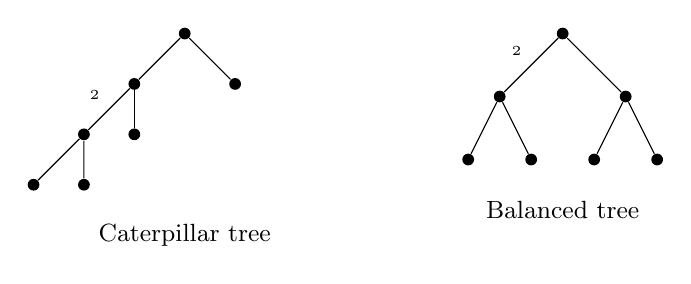
\begin{tikzpicture}[scale=0.8]

% Caterpillar
\begin{scope}[xshift=-3cm]
\node[circle, fill=black, inner sep=1.5pt] (root) at (0,0) {};
\node[circle, fill=black, inner sep=1.5pt] (n1) at (-0.8,-0.8) {};
\node[circle, fill=black, inner sep=1.5pt] (n2) at (0.8,-0.8) {};
\node[circle, fill=black, inner sep=1.5pt] (n3) at (-1.6,-1.6) {};
\node[circle, fill=black, inner sep=1.5pt] (n4) at (-0.8,-1.6) {};
\node[circle, fill=black, inner sep=1.5pt] (n5) at (-2.4,-2.4) {};
\node[circle, fill=black, inner sep=1.5pt] (n6) at (-1.6,-2.4) {};

\draw (root) -- (n1);
\draw (root) -- (n2);
\draw (n1) -- (n3) node[midway, above left] {\tiny 2};
\draw (n1) -- (n4);
\draw (n3) -- (n5);
\draw (n3) -- (n6);

\node at (0,-3.2) {\small Caterpillar tree};
\end{scope}

% Balanced
\begin{scope}[xshift=3cm]
\node[circle, fill=black, inner sep=1.5pt] (root) at (0,0) {};
\node[circle, fill=black, inner sep=1.5pt] (n1) at (-1,-1) {};
\node[circle, fill=black, inner sep=1.5pt] (n2) at (1,-1) {};
\node[circle, fill=black, inner sep=1.5pt] (n3) at (-1.5,-2) {};
\node[circle, fill=black, inner sep=1.5pt] (n4) at (-0.5,-2) {};
\node[circle, fill=black, inner sep=1.5pt] (n5) at (0.5,-2) {};
\node[circle, fill=black, inner sep=1.5pt] (n6) at (1.5,-2) {};

\draw (root) -- (n1) node[midway, above left] {\tiny 2};
\draw (root) -- (n2);
\draw (n1) -- (n3);
\draw (n1) -- (n4);
\draw (n2) -- (n5);
\draw (n2) -- (n6);

\node at (0,-2.8) {\small Balanced tree};
\end{scope}
\end{tikzpicture}

\caption{The two main extremal tree topologies: caterpillar and balanced trees.}

\label{fig:caterpillar_and_balanced_tree}
\end{figure}
% end fig

\vspace{0.5em}



\note{

  With these bottlenecks in mind, lets introduce the two main topologies of interest.\\

  \vspace{0.5em}

  First, we have caterpillar trees, which are basically just this long spine with single leaves branching off at each point. These trees have
  many large bipartitions, and represent our combinatorially bottleneck. 

  \vspace{0.5em}

  Second, we have balanced trees. These are trees where for every vertex $v$, the 
  number of leaves in its left and right subtrees differ only by at most one. These trees make coalescence difficult because: (i) lineages
  are so evenly spread out they cannot take advantage of the quadratic coalescent rates of Kingman's coalescent and (ii) leaves are separated from
  the root by as few edges as possible, so each lineage has very little time to coalesce. Hence these trees represent our coalescent bottleneck. \\

  \vspace{0.5em}

  \noindent In a sense, these are the two extremes of the space of trees: one maximally balanced and the other maximally imbalanced.
}
\end{frame}

\begin{frame}{Caterpillar Bound}

  % Example alpha_i
\begin{figure}[h]
\centering
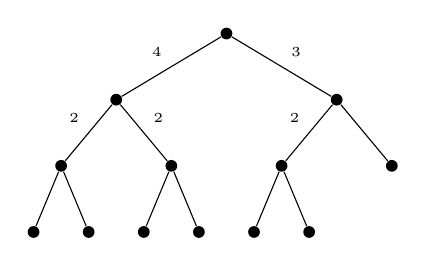
\begin{tikzpicture}[scale=0.7]

\node[circle, fill=black, inner sep=1.5pt] (root) at (0,0) {};
\node[circle, fill=black, inner sep=1.5pt] (n1) at (-2,-1.2) {};
\node[circle, fill=black, inner sep=1.5pt] (n2) at (2,-1.2) {};
\node[circle, fill=black, inner sep=1.5pt] (n3) at (-3,-2.4) {};
\node[circle, fill=black, inner sep=1.5pt] (n4) at (-1,-2.4) {};
\node[circle, fill=black, inner sep=1.5pt] (n5) at (1,-2.4) {};
\node[circle, fill=black, inner sep=1.5pt] (n6) at (3,-2.4) {};
\node[circle, fill=black, inner sep=1.5pt] (n7) at (-3.5,-3.6) {};
\node[circle, fill=black, inner sep=1.5pt] (n8) at (-2.5,-3.6) {};
\node[circle, fill=black, inner sep=1.5pt] (n9) at (-1.5,-3.6) {};
\node[circle, fill=black, inner sep=1.5pt] (n10) at (-0.5,-3.6) {};
\node[circle, fill=black, inner sep=1.5pt] (n11) at (0.5,-3.6) {};
\node[circle, fill=black, inner sep=1.5pt] (n12) at (1.5,-3.6) {};

\draw (root) -- (n1) node[midway, above left] {\tiny 4};
\draw (root) -- (n2) node[midway, above right] {\tiny 3};
\draw (n1) -- (n3) node[midway, above left] {\tiny 2};
\draw (n1) -- (n4) node[midway, above right] {\tiny 2};
\draw (n2) -- (n5) node[midway, above left] {\tiny 2};
\draw (n2) -- (n6);
\draw (n3) -- (n7);
\draw (n3) -- (n8);
\draw (n4) -- (n9);
\draw (n4) -- (n10);
\draw (n5) -- (n11);
\draw (n5) -- (n12);
\end{tikzpicture}
\caption{Example of the descendant counts $\{\alpha_i\}$ associated to the nontrivial bipartitions/edges. }
\label{fig:example_descendants_alpha_i}
\end{figure}
% end fig


\begin{lemma}
    If $1 < \alpha_1 \leq \ldots \leq \alpha_{k-3}$ are the descendant counts of any phylogenetic tree, then $\alpha_i \leq i+1$. In particular,
    if $f:\mathbb{N} \to \mathbb{R}$ is increasing then: 
    \[\sum_{i=1}^{k-3} f(\alpha_i) \leq \sum_{i=2}^{k-2} f(i)\]
\end{lemma}

\note{
  Now let's make it precise what we mean by "caterpillar trees have many large bipartitions". 
  Given an edge $e$, define its \textit{descendant count} $\alpha_e$ to be the number of leaves in the subtree below $e$. Here's an example in
  the figure above. \\

  \vspace{0.5em}

  For a caterpillar tree, its easy to see the descendant counts of the nontrivial edges/bipartitions are $\{2,3\ldots k-2\}$. The
  following lemma says that we can pair up the edges in any tree $\mathcal{T}$ with those of a caterpillar tree in a way so that
  the descendant counts of $\mathcal{T}$ are at most those of the caterpillar tree. \\

  \vspace{0.5em}
  The result is more or less obvious and just requires a little book-keeping, but it quantifies our notion
  of a combinatorial bottleneck. 


}
\end{frame}

%%%%%%%%%%%%%%%%%%%%%%%%%%%%%%%%%%%%%%%%%%%%%%%%%%
% Balanced Trees Minimize Coalescence %
%%%%%%%%%%%%%%%%%%%%%%%%%%%%%%%%%%%%%%%%%%%%%%%%%%

\begin{frame}{Balanced Trees Minimize Coalesence}

  \textit{FOSD}: Given $X,Y$ we say $X \leq_{st} Y$ if $\mathbb{E}\phi(X) \leq \mathbb{E}\phi(Y)$ for all increasing functions $\phi$.\\
  
  \vspace{0.5em}


  Let $X_{\mathcal{T}}$ be the number of lineages reaching the root of a tree $\mathcal{T}$ under the MSC model.

  \begin{theorem}
    If $\mathcal{T}$ has $k$ leaves and minimum branch length $t_{min}$, then:
    %
    \[X_{\mathcal{T}} \leq_{st} X_{\mathcal{B}_{k, t_{min}}}\]
    %
    \noindent where $\mathcal{B}_{k,t}$ is the balanced tree with $k$ leaves and all branch lengths equal to $t_{min}$. 
  \end{theorem}

  \noindent As $g_{\ell,1}(t)$ is a decreasing function of $\ell$, we see:
  %
  \[p_e := \mathbb{E} g_{X_e, 1}(t_e) \geq \mathbb{E} g_{W_e, 1}(t_{min}), \quad W_e := X_{\mathcal{B}_{k_e, t_{min}}}. \]
  %
  
  \note{
    Next, we make precise what we mean by "balanced trees minimize coalescence".\\

    \vspace{0.5em}
    To do so, we need a notion of when one random variable is larger than other. Here, we
    rely on the standard notion of first-order stochastic dominance, which says $X \leq_{st} Y$ if for any increasing test function
    $\phi$, we have $\mathbb{E}\phi(X) \leq \mathbb{E}\phi(Y)$.\\
    
    \vspace{0.5em}
    With this in mind, let $X_{\mathcal{T}}$ be the number of lineages reaching the root of a tree $\mathcal{T}$ under the MSC model. 
    The following theorem says that for any tree $\mathcal{T}$ with $k$ leaves and minimum branch length $t_{min}$, we 
    have $X_{\mathcal{T}} \leq_{st} X_{\mathcal{B}_{k, t_{min}}}$, where $\mathcal{B}_{k,t}$ is the balanced tree with $k$ leaves and all branch lengths equal to $t_{min}$.
    Namely, more lineages tend to remain uncoalesced in the balanced tree than under any other topology.\\

     \vspace{0.5em}
     Since $g_{\ell,1}(t)$ is a decreasing function of $\ell$, this implies that the probability of absorption $p_e$ is at least as large as the case where we have a balanced tree with branch lengths as short as possible.
    In words, the probability a bipartition corresponding to an edge $e$ appears 
    is at worst that of the case where the subtree below this edge is balanced with 
    branch lengths as short as possible.

    Heuristically, balanced trees ought to minimize the amount of coalescence
    as lineages are spread as thinly apart as possible, and have as little distance as possible to travel to the root. 
    Since Kingman's coalescent rate is strongly convex in the number of lineages, its better that
    all lineages are close to the root rather than "some near and some far" (e.g. caterpillars)

  }
  
\end{frame}


%%%%%%%%%%%%%%%%%%%%%%%%%%%%%%%%%%%%%%%%%%%%%%%%%%
% Proof Sketch %
%%%%%%%%%%%%%%%%%%%%%%%%%%%%%%%%%%%%%%%%%%%%%%%%%%

\begin{frame}{Proof Outline}

  By induction on $k$, we see $X_{\mathcal{T}} \leq_{st} X_{\mathcal{T'}}$ where $\mathcal{T'}$ replaces subtrees of root with balanced trees:
  
  \vspace{0.5em}
  \begin{center}
    \begin{minipage}{0.45\linewidth}
      \centering
      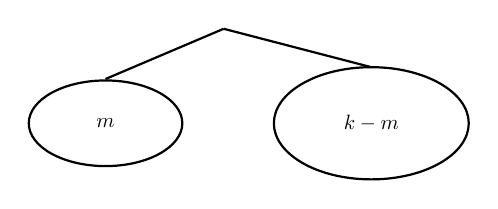
\begin{tikzpicture}[scale=0.75, transform shape, thick]
        % Define coordinates
        \coordinate (root) at (0, 1.6);
        \coordinate (left_child) at (-2.0, 0);
        \coordinate (right_child) at (2.5, 0);

        % Draw branches to left and right subtrees
        \draw (root) -- (-2.0, 0.75);
        \draw (root) -- (2.5, 0.95);

        % Draw the left subtree (smaller oval containing m)
        \node[draw, ellipse, minimum width=2.6cm, minimum height=1.45cm] at (left_child) {};
        \node at (left_child) {$m$};

        % Draw the right subtree (larger oval containing k-m)
        \node[draw, ellipse, minimum width=3.3cm, minimum height=1.9cm] at (right_child) {};
        \node at (right_child) {$k-m$};
      \end{tikzpicture}
    \end{minipage}
    \hfill
    \begin{minipage}{0.08\linewidth}
      \centering
      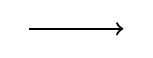
\begin{tikzpicture}[thick]
        \draw[->] (0,0) -- (1.2,0);
      \end{tikzpicture}
    \end{minipage}
    \hfill
    \begin{minipage}{0.45\linewidth}
      \centering
      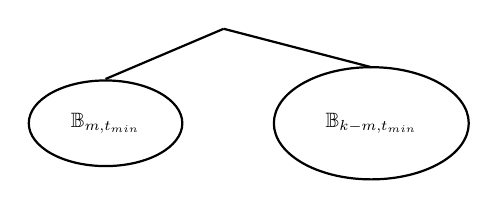
\begin{tikzpicture}[scale=0.75, transform shape, thick]
        % Define coordinates
        \coordinate (root) at (0, 1.6);
        \coordinate (left_child) at (-2.0, 0);
        \coordinate (right_child) at (2.5, 0);

        % Draw branches to left and right subtrees
        \draw (root) -- (-2.0, 0.75);
        \draw (root) -- (2.5, 0.95);

        % Draw the left subtree (smaller oval containing m)
        \node[draw, ellipse, minimum width=2.6cm, minimum height=1.45cm] at (left_child) {};
        \node at (left_child) {$\mathbb{B}_{m, t_{min}}$};

        % Draw the right subtree (larger oval containing k-m)
        \node[draw, ellipse, minimum width=3.3cm, minimum height=1.9cm] at (right_child) {};
        \node at (right_child) {$\mathbb{B}_{k-m, t_{min}}$};
      \end{tikzpicture}
    \end{minipage}
  \end{center}

  \vspace{0.5em}

  % end figure
  \noindent Next, we want to rebalance the subtrees so they have the same size: 

  \vspace{0.4em}
  \begin{center}
    \begin{minipage}{0.45\linewidth}
      \centering
      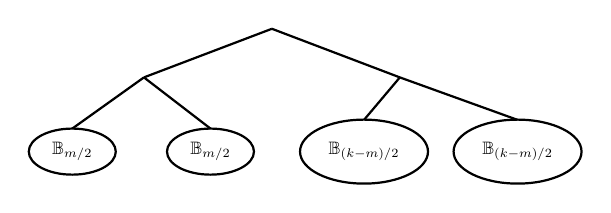
\begin{tikzpicture}[scale=0.65, transform shape, thick]
        % Internal binary-tree structure
        \coordinate (root) at (0, 2.4);
        \coordinate (left_child) at (-2.5, 1.45);
        \coordinate (right_child) at (2.5, 1.45);

        % Centers of bottom ovals (one layer deeper)
        \coordinate (ll) at (-3.9, 0.0);
        \coordinate (lr) at (-1.2, 0.0);
        \coordinate (rl) at (1.8, 0.0);
        \coordinate (rr) at (4.8, 0.0);

        % Connection points at top of each oval
        \coordinate (ll_top) at (-3.9, 0.45);
        \coordinate (lr_top) at (-1.2, 0.45);
        \coordinate (rl_top) at (1.8, 0.62);
        \coordinate (rr_top) at (4.8, 0.62);

        % Draw branches
        \draw (root) -- (left_child);
        \draw (root) -- (right_child);
        \draw (left_child) -- (ll_top);
        \draw (left_child) -- (lr_top);
        \draw (right_child) -- (rl_top);
        \draw (right_child) -- (rr_top);

        % Bottom subtrees as ovals
        \node[draw, ellipse, minimum width=1.7cm, minimum height=0.9cm] at (ll) {};
        \node at (ll) {$\mathbb{B}_{m/2}$};
        \node[draw, ellipse, minimum width=1.7cm, minimum height=0.9cm] at (lr) {};
        \node at (lr) {$\mathbb{B}_{m/2}$};
        \node[draw, ellipse, minimum width=2.5cm, minimum height=1.25cm] at (rl) {};
        \node at (rl) {$\mathbb{B}_{(k-m)/2}$};
        \node[draw, ellipse, minimum width=2.5cm, minimum height=1.25cm] at (rr) {};
        \node at (rr) {$\mathbb{B}_{(k-m)/2}$};
      \end{tikzpicture}
    \end{minipage}
    \hfill
    \begin{minipage}{0.08\linewidth}
      \centering
      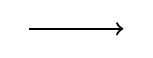
\begin{tikzpicture}[thick]
        \draw[->] (0,0) -- (1.2,0);
      \end{tikzpicture}
    \end{minipage}
    \hfill
    \begin{minipage}{0.45\linewidth}
      \centering
      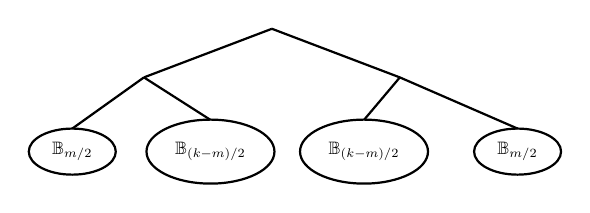
\begin{tikzpicture}[scale=0.65, transform shape, thick]
        % Internal binary-tree structure
        \coordinate (root) at (0, 2.4);
        \coordinate (left_child) at (-2.5, 1.45);
        \coordinate (right_child) at (2.5, 1.45);

        % Centers of bottom ovals (one layer deeper)
        \coordinate (ll) at (-3.9, 0.0);
        \coordinate (lr) at (-1.2, 0.0);
        \coordinate (rl) at (1.8, 0.0);
        \coordinate (rr) at (4.8, 0.0);

        % Connection points at top of each oval
        \coordinate (ll_top) at (-3.9, 0.45);
        \coordinate (lr_top) at (-1.2, 0.62);
        \coordinate (rl_top) at (1.8, 0.62);
        \coordinate (rr_top) at (4.8, 0.45);

        % Draw branches
        \draw (root) -- (left_child);
        \draw (root) -- (right_child);
        \draw (left_child) -- (ll_top);
        \draw (left_child) -- (lr_top);
        \draw (right_child) -- (rl_top);
        \draw (right_child) -- (rr_top);

        % Bottom subtrees as ovals
        \node[draw, ellipse, minimum width=1.7cm, minimum height=0.9cm] at (ll) {};
        \node at (ll) {$\mathbb{B}_{m/2}$};
        \node[draw, ellipse, minimum width=2.5cm, minimum height=1.25cm] at (lr) {};
        \node at (lr) {$\mathbb{B}_{(k-m)/2}$};
        \node[draw, ellipse, minimum width=2.5cm, minimum height=1.25cm] at (rl) {};
        \node at (rl) {$\mathbb{B}_{(k-m)/2}$};
        \node[draw, ellipse, minimum width=1.7cm, minimum height=0.9cm] at (rr) {};
        \node at (rr) {$\mathbb{B}_{m/2}$};
      \end{tikzpicture}
    \end{minipage}
  \end{center}



  \note{
    Let's outline the proof at a high-level. We start by reducing to the case where the subtrees of the root are balanced. This is done by applying the inductive hypothesis to each subtree of the root separately.\\
    
    \vspace{0.5em}
    Next, we want to rebalance the subtrees so they have the same size. Heuristically, this
    works because Kingman's coalescent rate is strongly convex in the number of lineages. Using the recursive structure
    of the balanced tree, we know its subtrees are again balanced.

    \vspace{0.5em}
    Then the result follows by again applying the inductive hypothesis to each subtree of the root separately.\\

    \vspace{0.5em}
    So all that is left to verify is that when we perform this local rebalancing step, we are no worse off then before.\\

    \vspace{0.5em}
    The same argument above works without reducing to balanced subtrees, but its easier to verify some of the
    conditions of our lemmas below for balanced subtrees. We are essentially just starting at the leaves
    and balancing each vertex as we work our way up to the root.
  }
\end{frame}


%%%%%%%%%%%%%%%%%%%%%%%%%%%%%%%%%%%%%%%%%%%%%%%%%%
% Deterministic Balancing Lemma %
%%%%%%%%%%%%%%%%%%%%%%%%%%%%%%%%%%%%%%%%%%%%%%%%%%
\begin{frame}{Deterministic Balancing Lemma}

  Let $Z_i^t$ have distribution $\mathbb{P}(Z_i^t = j) = g_{ij}(t)$. 

  \vspace{0.5em}

 
  \begin{lemma}[Deterministic Balancing Lemma]
    %
    Fix $k \in \mathbb{N}$. For $1 \leq i \leq j \leq \lfloor \frac{k}{2} \rfloor$:
    \[Z^t_{i} + Z_{k-i}^t \leq_{st} Z^t_{j} + Z_{k-j}^t \]
    %
  \end{lemma}


\begin{center}
  \begin{minipage}{0.41\linewidth}
    \centering
    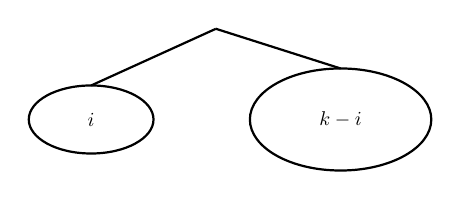
\begin{tikzpicture}[scale=0.72, transform shape, thick]
      % Define coordinates
      \coordinate (root) at (0, 1.6);
      \coordinate (left_child) at (-2.2, 0);
      \coordinate (right_child) at (2.2, 0);
      \coordinate (left_top) at (-2.2, 0.6);
      \coordinate (right_top) at (2.2, 0.9);

      % Draw branches to left and right subtrees
      \draw (root) -- (left_top);
      \draw (root) -- (right_top);

      % Draw the left subtree (oval containing m)
      \node[draw, ellipse, minimum width=2.2cm, minimum height=1.2cm] at (left_child) {};
      \node at (left_child) {$i$};

      % Draw the right subtree (oval containing k-m)
      \node[draw, ellipse, minimum width=3.2cm, minimum height=1.8cm] at (right_child) {};
      \node at (right_child) {$k-i$};
    \end{tikzpicture}
  \end{minipage}
  \hspace{0.03\linewidth}
  \begin{minipage}{0.41\linewidth}
    \centering
    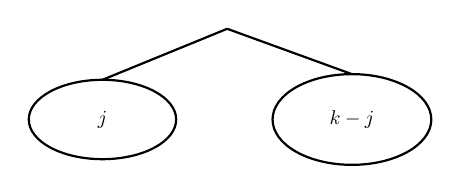
\begin{tikzpicture}[scale=0.72, transform shape, thick]
      % Define coordinates
      \coordinate (root) at (0, 1.6);
      \coordinate (left_child) at (-2.2, 0);
      \coordinate (right_child) at (2.2, 0);
      \coordinate (left_top) at (-2.2, 0.7);
      \coordinate (right_top) at (2.2, 0.8);

      % Draw branches to left and right subtrees
      \draw (root) -- (left_top);
      \draw (root) -- (right_top);

      % Draw the left subtree (oval containing m): slightly larger
      \node[draw, ellipse, minimum width=2.6cm, minimum height=1.4cm] at (left_child) {};
      \node at (left_child) {$j$};

      % Draw the right subtree (oval containing k-m): slightly smaller
      \node[draw, ellipse, minimum width=2.8cm, minimum height=1.6cm] at (right_child) {};
      \node at (right_child) {$k-j$};
    \end{tikzpicture}
  \end{minipage}
\end{center}

  \note{
   \textbf{Goal:} Justify this rebalancing operation can only make coalescence worse.\\

   \vspace{0.5em}

   Let's start with the simpler case where the subpopulations are deterministic. Namely, we aim to show
   (read lemma and go over picture). Heuristically it says the more balanced these two subpopulations are
   below the given edge, the more lineages tend to reach that edge. \\


   }
  
\end{frame}

\begin{frame}{Proof Outline}
  
  \textbf{Deterministic Balancing Lemma:}

  \begin{itemize}
    \item Condition on time of first coalescent event; more balanced $=$ longer wait.
          \[\text{rate} = {i \choose 2} + {k-i \choose 2}\]

    \item Rely on monotonicity with respect to $t$: for $t < t'$, $Z_i^t \geq_{st} Z_i^{t'}$.

    \item After first coalescent event, imbalance can only change by one. Hence if $i < j < \lfloor k/2\rfloor$ 
          starts more imbalanced, it must tend to stay that way. 
    
    \[(i, k-i) \text{ with imbalance } k-2i\to \begin{cases} (i-1, k-i) & \text{ with imbalance } k-2i + 1 \\
       (i, k-i-1) & \text{ with imbalance } k-2i-1 \end{cases}\]


  \end{itemize}

  \note{
    The proof of this first balancing lemma is relatively straightforward. (go over proof outline)
    Basically, because the coalescent rate is convex in the number of lineages (its quadratic) 
    the total rate is minimized when the two subpopulations are as balanced as possible. Hence, the more balanced we start, the longer we 
    expect to wait until the first coalescent event.\\
    
    \vspace{0.5em}

    Moreover, after the first coalescent event, the imbalance between the two subpopulations can only change by one,
    so if we start more imbalanced, we tend to stay more imbalanced. \\
    
    
    \vspace{0.5em}
    Finally, we rely on monotonicity with respect to $t$. Namely, having more time to coalesce can only reduce
    the number of lineages reaching the root.

  }
\end{frame}

%%%%%%%%%%%%%%%%%%%%%%%%%%%%%%%%%%%%%%%%%%%%%%%%%%
% Balancing Lemma %
%%%%%%%%%%%%%%%%%%%%%%%%%%%%%%%%%%%%%%%%%%%%%%%%%%


\begin{frame}{Balancing Lemma}

  Now extend to a random number of initial lineages.

  \vspace{0.5em}

  \textit{Likelihood Ratio Order:} We say $X \leq_{lr} Y$ if:
  %
  \[\frac{\mathbb{P}(X = k)}{\mathbb{P}(Y=k)}\]
  %
  \noindent is non-decreasing in $k$. Note $X \leq_{lr} Y$ implies $X \leq_{st} Y$.

  \begin{lemma}[Balancing Lemma]

    If $A \leq_{lr} A'$ and $B \leq_{lr} B'$, and $A,B,A',B'$ are mutually independent then:
    %
      \[Z^t_{A + B} + Z^t_{A' + B'} \leq_{st} Z^t_{A + B'} + Z^t_{A' + B}\]
    %
  \end{lemma}

\note{
  Now we would like to extend the previous lemma to allow for a \textit{random} number of initial lineages. 
  This is important because when we perform the rebalancing operation, the number of lineages in each subtree is random.\\

  \vspace{0.5em}
  To do so, we again need a notion of when the two (random) subpopulations of the root are imbalanced. For the proof, we need
  a stronger stochastic order than FOSD. In particular, we say $X \leq_{lr} Y$ (read the definition). Note $X \leq_{lr} Y$ implies $X \leq_{st} Y$.\\

  \vspace{0.5em}
  (read balancing lemma). Heuristically, this says that if we have 4 random subpopulations, two larger and two smaller,  
  pairing a smaller one with a larger one will tend to increase the number of lineages reaching the root. 
}
\end{frame}


\begin{frame}{Proof Outlines}

  \textbf{Balancing Lemma:}
  \begin{itemize}
    \item Rephrase deterministic lemma in terms of sums/differences: if $0 \leq d \leq d' < s$ then:
          \[Z^t_{\frac{s-d'}{2}} + Z^t_{\frac{s+d'}{2}} \leq_{st} Z^t_{\frac{s-d}{2}} + Z^t_{\frac{s+d}{2}}\]

    \item Extend to random differences: if $0 \leq_{st} D \leq_{st} D' \leq_{st} s$ then $\ldots$ 
    \item Define pairwise sums/differences
         \[\Delta_A := A' - A, \quad \Delta_B := B' - B, \quad S_A := A' + A, \quad S_B = B' + B.\]

    \item Apply previous with conditional differences:
     %
      \[D' = |\Delta_A + \Delta_B| \mid \{|\Delta_A|, |\Delta_B| , S_A, S_B \}, \qquad D = |\Delta_A - \Delta_B| \mid \{|\Delta_A|, |\Delta_B| , S_A, S_B \}.\]
     %
     \item After conditioning  $\{D, D'\} = \{|\Delta_A| + |\Delta_B|, ||\Delta_A| - |\Delta_B||\}$.
  \end{itemize}

  \note{

    The proof basically boils down to careful conditioning on the total number of lineages, and then controlling
    the imbalance between the two subpopulations of the root in the two different settings. \\

    \vspace{0.5em}
    Formally, we can rephrase the deterministic lemma in terms of total number of lineages $s$ across the two subpopulations
    and the difference $d$ in size between the two subpopulations. This maybe makes it a bit more concrete what we mean by
    "more balanced".\\

    \vspace{0.5em}
    From here, its easy to extend this to random imbalanced $D,D'$. \\

    \vspace{0.5em}
    The balancing lemma then follows by conditioning on the total number of lineages and applying this 
    idea to the conditional differences defined as shown on the screen. After conditioning, these 
    differences are particularlly simple, and its easy to verify the likelihood ratio ordering gives us what we want. 


  }
  

  
\end{frame}



%%%%%%%%%%%%%%%%%%%%%%%%%%%%%%%%%%%%%%%%%%%%%%%%%%
% Bipartition Cover Bound %
%%%%%%%%%%%%%%%%%%%%%%%%%%%%%%%%%%%%%%%%%%%%%%%%%%

\begin{frame}{Bipartition Cover Bound}

  Combining our above results gives:

  \begin{corollary}[Bipartition Cover Bound]
    Given $n$ gene trees sampled independently under the MSC model from a species 
    tree $\mathcal{T}$ with $k$ species and minimum branch length $t_{min}$, then:
    %
    \[\mathbb{P}(\text{cover}) \geq 1-\sum_{\ell=2}^{k-2}(1-w_\ell)^n\]
    %
    \noindent where $w_\ell := \mathbb{E} g_{W_\ell, 1}(t_{min})$ for $W_\ell := X_{\mathcal{B}_{\ell, t_{min}}}$.
  \end{corollary}

  \noindent Due to recursive structure, distributions of $W_\ell$ are easy to compute dynamically.
  

\note{
  Combining our analysis of caterpillar and balanced trees, we can produce our bipartition cover bound. 
  (read theorem). \\

  \vspace{0.5em}
  The caterpillar bound determines the descendant counts we are using in our sum, and the balanced tree bound determines 
  the distribution of lineages we are using to compute the $w_\ell$'s.\\
  %

  \vspace{0.5em}
  While this bound is only implicit in $n$, due to the recursive structure of balanced trees the
  distributions of $W_\ell$ are easy to compute dynamically, so we can easily get numerical estimates of the bound for any given $n$.
}


\end{frame}

%%%%%%%%%%%%%%%%%%%%%%%%%%%%%%%%%%%%%%%%%%%%%%%%%%
% Empirical Results %
%%%%%%%%%%%%%%%%%%%%%%%%%%%%%%%%%%%%%%%%%%%%%%%%%%

\section{Empirical Results}

\begin{frame}{Empirical Results}
  \noindent Fix $q \in (0,1)$. Let $n_q$ be the smallest $n$ that ensures $\mathbb{P}(\text{cover}) \geq q$ under our bound.
\begin{center}
  
\includegraphics[width=0.9\linewidth]{figures/balanced_bound.png}
\end{center}

\begin{itemize}
  \item Sharply sensitive to small $t_{min}$. 
  \item Mostly saturates as a function of $k$ past some point.  
\end{itemize}


\note{
  Since our bound is sort of a complicated function of its two key parameters $k, t_{min}$, lets try to
  first empirically explore how it behaves. First, we just start by choosing some coverage probability $q \in (0,1)$ and
  plotting the smallest $n_q$ under which our bound ensures $\mathbb{P}(\text{cover}) \geq q$ as a function of $k$ and $t_{min}$.\\

  \vspace{0.5em}

  We can observe two things. For one, the bound is sharply sensitive to small values of $t_{min}$, growing rapidly when
  this parameter is near zero. In our next section, we can relate this to the behavior of $g_{\ell, 1}(T)$ near $T=0$. \\

  \vspace{0.5em}

  Next, we see that the bound mostly saturates as a function of $k$ past some point. This is likely because of the strong coalescent 
  properties of Kingman's coalescent: the behavior of our bound is sort of dominated by the hardest bipartition to recover 
  , and at some point increasing the number of lineages below its corresponding edge will barely change the number of lineages that tends to reach it. , increasing $k$ just adds more bipartitions that are near saturation and behave similarly under our framework.
  So we really only pick up a $\log(k)$ factor from the number of species by adding another term to our sum. 


}

\end{frame}

\begin{frame}{Overestimation Ratios}
  
  Empirically estimate true $q^{th}$ quantile $n_q^*$ for:
  \begin{itemize}
    \item Caterpillar trees with all branch lengths equal to $t_{min}$.
    \item Balanced trees with all branch lengths equal to $t_{min}$.
  \end{itemize}

  \noindent Then we plot the \textit{overestimation ratio} $\frac{n_q}{n_q^*}$ as a function of $k, t_{min}$.\\

  \vspace{0.5em}
  To get a sense of performance of our bound on a "typical" tree we:
  
  \begin{itemize}
    \item Simulate many random Yule trees.
    \item Estimate $n_q^*$ for each tree via simulation.
    \item Study distribution of $\frac{n_q}{n_q^*}$ across trees. 
  \end{itemize}


\end{frame}

\begin{frame}{Overestimation Ratios: Caterpillar}

  \begin{center}
    \includegraphics[width=0.98\linewidth,height=0.78\textheight,keepaspectratio]{figures/overestimation_caterpillar.png}
  \end{center}

\end{frame}

\begin{frame}{Overestimation Ratios: Balanced}

  \begin{center}
    \includegraphics[width=0.98\linewidth,height=0.78\textheight,keepaspectratio]{figures/overestimation_balanced.png}
  \end{center}

\end{frame}

\begin{frame}{Overestimation Ratios: Yule Trees}

  \begin{center}
    \begin{minipage}{0.49\linewidth}
      \centering
      \includegraphics[width=\linewidth,height=0.68\textheight,keepaspectratio]{figures/overestimation_yule_1.png}
    \end{minipage}
    \hfill
    \begin{minipage}{0.49\linewidth}
      \centering
      \includegraphics[width=\linewidth,height=0.68\textheight,keepaspectratio]{figures/overestimation_yule_2.png}
    \end{minipage}
  \end{center}

\end{frame}


%%%%%%%%%%%%%%%%%%%%%%%%%%%%%%%%%%%%%%%%%%%%%%%%%%
% Asymptotic Analysis %
%%%%%%%%%%%%%%%%%%%%%%%%%%%%%%%%%%%%%%%%%%%%%%%%%%

\section{Asymptotic Analysis}

\begin{frame}{Asymptotic Analysis}

  \noindent We are interested in the regime where:
\begin{itemize}
  \item The number of species $k$ is large. 
  \item The minimum branch length $t_{\min}$ is small.
\end{itemize}

\vspace{0.6em}

\noindent Since $n_q$ is only an implicit function of $k, t_{min}$, we upper bound it by observing:
%
\begin{itemize}
  \item $g_{\ell, 1}(t)$ is convex in $\ell$. 
  \item We can upper bound $\mathbb{E} W_\ell \leq \frac{2-e^{-t_{min}/2}}{1-e^{-t_{min}/2}} \asymp 2t_{min}^{-1} $. Reasonable for large $k$. 
\end{itemize}

\noindent Hence: 

\[\sum_{\ell=2}^{k-2} (1-w_\ell)^n \leq (k-3)(1-w_{k-2})^n \Rightarrow n_q \lesssim \frac{\log\left(\frac{1-q}{k-3}\right)}{\log(1-g_{2t^{-1}, 1}(t))}\]
%


\note{
  Our bound is sort of complicated, but we can derive some asymptotics using some asymptotic properties of the
  absorption probabilities $g_{\ell, 1}(t)$. The main regime we care about is when the number of species $k$
  is large and the minimal branch length $t_{min}$ is small.\\
  
  \vspace{0.5em}
  Using some basical properties of $g_{\ell,1}$ we can get an upper bound on our bipartition cover
  bound $n_q$ in terms of $g_{2t^{-1}, 1}(t)$. This upper bound is at least reasonable when $k$ is large so we are close to saturation,
  and most terms in the sum are similar.\\
}
\end{frame}


%% Asymptotics of Kingmans coalescent absorption probabilities %%%%%
\begin{frame}{Asymptotics of $g_{\ell, 1}(t)$}
 In the fixed $k$, small $t$ regime, we get polynomial decay in $t^{-1}$:
%
\[g_{\ell, 1}(t) \sim \frac{\ell!}{2^{\ell-1}} t^{\ell - 1}, \quad \ell^{-2} t \downarrow 0.\]
%
For fixed $t$ we saw $g_{\ell, 1}(t)$ saturates $s(t) := \lim_{\ell \to \infty} g_{\ell, 1}(t) > 0$ with gap:
%
\[\Delta_t(k) := g_{\ell, 1}(t) - s(t) =  \frac{2s'(t)}{\ell} + o(\ell^{-1})\]
%
\noindent Moreover, via classical Tauberian theory the limiting CDF $s(t)$ has small $t$ asymptotics:
%
\[s(t) = \exp \left(- \Theta(t^{-1})\right)\]
%
\note{
  To analyze our upper bound, we develop some asymptotics for $g_{\ell, 1}(t)$. These follow from simple Taylor expansions and hazard rate analysis.\\

  \vspace{0.5em}
  These bounds concretely display the strong dependence on the minimal branch length $t_{min}$. 
  In the small $t$ regime, we get polynomial decay in $t^{-1}$, with degree depending on $k$. 
  In the large $k$ regime, we see $g_{\ell, 1}(t)$ saturates to some limit $s(t)$ with gap $\Delta_t(k) \asymp \ell^{-1}$. Moreover, using classical Tauberian theory we can get small $t$ asymptotics for $s(t)$, which is the key quantity controlling the large $k$ behavior of our bound.\\
  Again this causes $k$ to really only appears up to a log factor.\\

  \vspace{0.5em}
  Lastly, we show that our limiting CDF $s(t)$ decays very strongly near zero. 
}
\end{frame}

%%%%%% Large k, small t behavior %%%%%%%%%
\begin{frame}{Large $k$, Small $t_{min}$ Behavior}

Suppose $t_{min}$ is fixed. Let $h_t := g_{2t^{-1}, 1}(t)$ and $\Delta = h_t - s(t)$. Above we saw for large $k$:
%
\[n_q \lesssim \frac{\log(k)}{-\log(1-h_t)} \approx \frac{\log(k)}{s(t) \left(1 + \frac{\Delta}{s(t)}\right)} \]
%
\noindent Some simple rearragements shows:
%
\[\frac{\Delta}{s(t)} \approx t \cdot \frac{d}{dt} \log s(t) \approx t^{-1}\]
%
\noindent so roughly:
%
\[n_q \lesssim \log(k) t \exp(\Theta(t^{-1}))\] 
%
\note{
  Using these asymptotics, some simple rearrangements and a bit of hand-waving show that in the large $k$, small $t$ regime, 
  our bound behaves at most like $\log(k) t \exp(\Theta(t^{-1}))$.\\

  \vspace{0.5em}
  So we sort of have a trade-off: if we want to use the full search space, it will take superexponentially long to run the optimization problem
  we are hoping to solve, but if we use the restricted search space we will need almost an exponential amount of data
  to get our desired coverage probability (although it runs in polynomial time).\\

  \vspace{0.5em}
  In practice, certain heuristics are used to expand the search space slightly which have 
  empirically been shown to be very effective at increasing the coverage probability. But from a theoretical 
  standpoint, we are still left with this trade-off.

}

\end{frame}





%%%%%%%%%%%%%%%%%%%%%%%%%%%%%%%%%%%%%%%%%%%%%%
% Conclusion 
%%%%%%%%%%%%%%%%%%%%%%%%%%%%%%%%%%%%%%%%%%%%%%
\section{Conclusion}

\begin{frame}{Takeaways}

\noindent \textbf{Takeaways:}
\begin{itemize}
  \item Caterpillars and balanced trees are the two main bottlenecks for bipartition recovery.
  \item Topology-free bounds are possible, but coarse; must account for \textit{both} extremes.
  \item Due to saturation in $k$, the minimal branch length $t_{min}$ is the key limiting factor.
\end{itemize}

\vspace{0.5em}

\noindent \textbf{Questions}:
\begin{itemize}
  \item Avoid union bound and take advantage of positive dependence?
  \item Extend to larger class of coalescent processes with sufficient "convexity"?
\end{itemize}

\note{
  In summary, we showed that when it comes to the MSC model, caterpillars and balanced trees are the two main bottlenecks for bipartition recovery. 
  Caterpillars are bad because they have a large number of lineages reaching the root, and balanced trees are bad because they tend to have a large number of lineages reaching the root.\\

  \vspace{0.5em}
  Using this, we constructed topology-free bounds on the bipartition coverage probability. Our topology-free framework, our "worst-case" is somehow simultaneously a caterpillar and also
  balanced tree, making it naturally somewhat coarse. Sharper bounds would likely require more specific topological assumptions.
  Nonetheless, our theoretical analysis showed this bipartition restricted search space can vastly increase the number of species
  on which phylogenetic inference can be reliably performed. \\

  \vspace{0.5em}
  Lastly, due to saturation in $k$, the minimal branch length $t_{min}$ is the key limiting factor for bipartition recovery. 
}
\end{frame}

\begin{frame}{Key References}
\footnotesize
\begin{thebibliography}{99}
\bibitem{uricchio2016}
Lawrence H. Uricchio, Tandy Warnow, and Noah A. Rosenberg.
\newblock An analytical upper bound on the number of loci required for all splits of a species tree to appear in a set of gene trees.
\newblock \emph{BMC Bioinformatics}, 17(Suppl 14):417, 2016.

\bibitem{shekhar2018}
Shameek Shekhar, Sebastien Roch, and Siavash Mirarab.
\newblock Species tree estimation using ASTRAL: how many genes are enough?
\newblock \emph{IEEE/ACM Transactions on Computational Biology and Bioinformatics}, 15(5):1738--1747, 2018.

\bibitem{mirarab2014}
Siavash Mirarab et al.
\newblock ASTRAL: genome-scale coalescent-based species tree estimation.
\newblock \emph{Bioinformatics}, 30(17):i541--i548, 2014.

\bibitem{rannala2020}
Bruce Rannala and Ziheng Yang.
\newblock The multispecies coalescent model and species tree inference.
\newblock In \emph{Phylogenetics in the Genomic Era}, chapter 3.3, 2020.
\end{thebibliography}


\note{

  Here are some of the key references for this work. Thank you all for listening to my talk. 

}

\end{frame}



\end{document}
